\documentclass{mwart}
%\usepackage{polski}
%\usepackage[polish]{babel}
\usepackage{amsfonts}
\usepackage{indentfirst}
\usepackage[utf8]{inputenc}
\usepackage{amsthm}
\usepackage{multirow}
\usepackage{amsmath}
\newtheorem{tw}{Twierdzenie}
\newtheorem{df}{Definicja}
\newtheorem{zd}{Zadanie}
\newtheorem{zdt}[zd]{Zadanie*}
\title{Zestaw 7}
\usepackage{Sweave}
\begin{document}
\Sconcordance{concordance:Zestaw7.tex:Zestaw7.Rnw:%
1 14 1 1 0 68 1 1 2 1 0 1 1 1 2 2 1 1 9 6 0 1 8 6 0 1 4 2 0 1 1 4 0 1 2 %
1 1}

\maketitle

\begin{zd}
Niech $(N_t)_{\{t \geq 0\}}$ będzie procesm Poissona z instensywnością 1.5. Oblicz:
\begin{itemize}
\item $\mathbb{P}(N_1=2, N_4=6)$,
\item $\mathbb{P}(N_5-N_2 = 3)$,
\item $\mathbb{P}(N_2+N_5=4)$,
\item $\mathbb{P}(N_4=6| N_1=2)$,
\item$\mathbb{P}(N_1=2| N_4=6)$.
\end{itemize}
\end{zd}

\begin{zd}
Niech $(N_t)_{\{t \geq 0\}}$ będzie procesm Poissona z instensywnością 2. Oblicz:
\begin{itemize}
\item $\mathbb{E}(N_3N_4)$,
\item $\mathbb{E}(S_3S_4)$,
\item $Var(N_5-2N_6+3N_{10})$,
\item $\mathbb{E}(N_5-2N_6+3N_{10})$,
\item $Cov(N_5-2N_6, 3N_{10})$,
\end{itemize}
gdzie $S_n$ jest $n$-tym czasem przybycia.
\end{zd}

\begin{zd}
Niech $N_t$ będzie procesem Poissona z intensywnością $\lambda$. Znajdź postać funkcji kowariancji tego procesu
\begin{displaymath}
C_N(t,s) = Cov(N_t, N_s)
\end{displaymath}
oraz funkcję autokorelacji tego procesu
\begin{displaymath}
	A_N(t,s) = \rho\left(N_t, N_s\right).
\end{displaymath}
\end{zd}

%poisson3.pdf proposition 6.1
\begin{zd}
Niech $(N_t)_{\{t \geq 0\}}$ będzie jednorodnym procesem Poissona z intensywnością $\lambda$. Dla $s > 0$ niech $\tilde{N}_t = N_{t+s} - N_s$ dla $t\geq 0$. Udowodnij, że $(\tilde{N}_t)_{\{t \geq 0\}}$ jest procesem Poissona z intensywnością $\lambda$.
\end{zd}

\begin{zd}
Niech $(N_t^1)_{\{t \geq 0\}}, (N_t^2)_{\{t \geq 0\}}, \dots, (N_t^k)_{\{t \geq 0\}}$ będą niezależnymi procesami Poissona z intensywnościami odpowiednio $\lambda^1$, $\lambda^2$, \dots, $\lambda^k$. Niech $N_t = N_t^1 + N_t^2 + \dots + N_t^k$ dla $t \geq 0$. Udowodnij, że wtedy $(N_t)_{\{t \geq 0\}}$ jest procesm Poissona o intensywności $\lambda = \lambda^1 + \lambda^2 + \dots + \lambda^k$.
\end{zd}

%poisson3.pdf Example 6.7
\begin{zd}
W kranine Oz spotkania z lwami, tygrysami i niedźwiedzami opisywane są procesami Poissona z intensywnościami odpowiednio $\lambda_l$, $\lambda_t$ i $\lambda_n$, gdzie jednostką czasu jest godzina. Spotaknie z każdym z gatunków jest niezależne od spotkania z pozostałymi.
\begin{itemize}
\item Jakie jest prowdopodobieństwo, że Dorotka nie spotka żadnego zwierzęcia w ciągu pierwszych 24 godzin od przybycia do krainy Oz?
\item Dorotka widziała 3 zwierzęta jednego dnia. Jakie jest prawdopodobieństwo, że widziała każdy z gatunków?
\end{itemize}
\end{zd}

%poisson3.pdf p.244
\begin{zd}
	Niech $N_t$ będzie procesem Poissona z intensywnością $\lambda$ i niech $X_1$ będzie czasem pierwszego przybycia. Pokaż, że warunkowo względem zdarzenia $N(t) = 1$, $X_1$ ma rozkład jednostajny na odcinku $(0,t]$, czyli
	\begin{displaymath}
	\mathbb{P}\left(X_1 \leq x|N(t) = 1\right) = \frac{x}{t},\ 0\leq x\leq t.
	\end{displaymath}
\end{zd}

%poisson3.pdf Example 6.13
\begin{zdt}[Niejednorodny proces Poissona] Studenci przybywają do stołówki zgodnie z niejednorodnym procesem Poissona. Częstość przybyć rośnie liniowo od 100 do 200 studentów między 11 a 12, następnie utrzymuje się na stałym poziomie do godziny 14, a następnie zmieniejsza się liniowo do 100 między 14 a 15. Jakie jest prawdopodobieństwo, że między 11:30 a 13:30 w stołówce będzie co najmniej 400 osób?

\end{zdt}

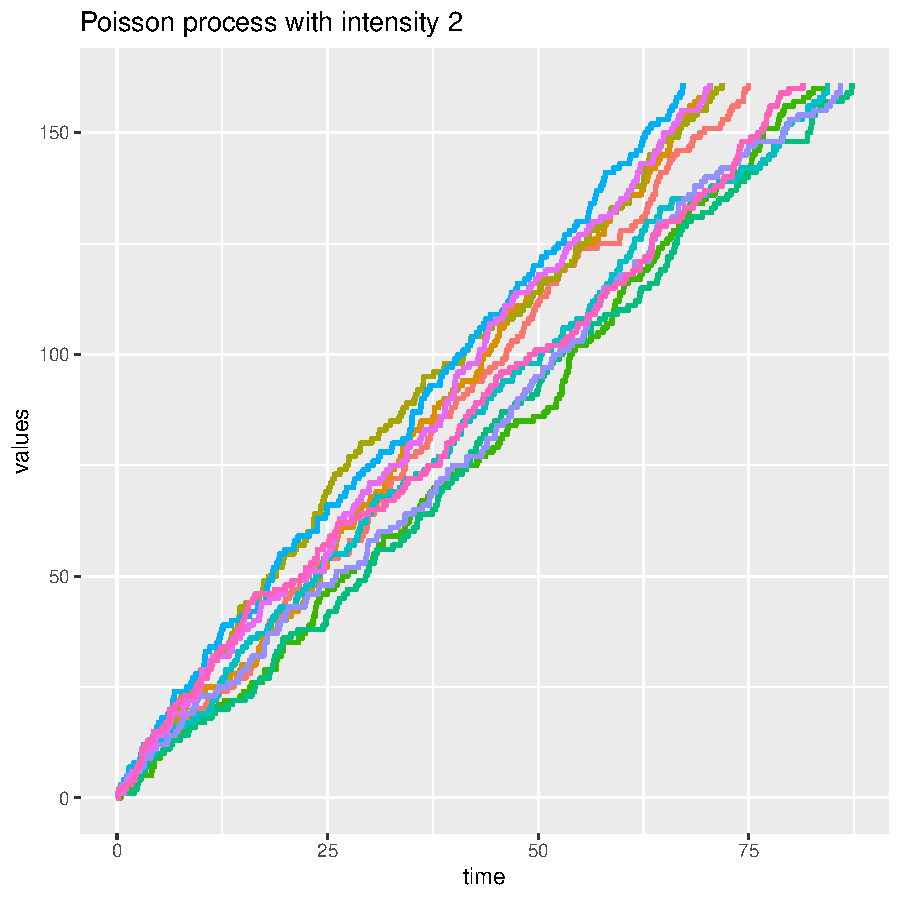
\includegraphics{Zestaw7-001}

\end{document}
